% !TEX root = ./paper.tex
\subsection{Methodology}

Our objective is to evaluate whether our design and implementation are indeed
fast, flexible and does not conflict with several commercial and open-source
middleboxes. Moreover, we expect to showcase and compare TCPLS's functionalities
such as the App-level connection migration, the failover mechanism or the
aggragation compability and discuss them  with the state
of the art designs, such as mvfst~\cite{mvfast}, quicly~\cite{quicly},
msquic~\cite{msquic}, MPTCP~\ref{mptcp}, pquic~\cite{pquic},
quic-go~\cite{quic-go} and MPQUIC~\ref{mpquic}.

%TODO do we also evelatuate security? with a simple proof and discussion?
To evaluate the performance (Section~\ref{sec:perf}) and middlebox traversal
(Section~\ref{sec:middlebox}), we deploy a testbed composed of three machines with Intel Xeon CPU E5-2630
2.40GHz, 16 Threads, at least 16GB RAM, running Debian with 5.9 and
5.7 kernels. Two of these machines play the role of Client and Server,
while one is the Network Simulator (NS). Each machine is equipped with an
Intel XL710 2x40GB NIC, directly connected as shown in
Fig.~\ref{fig:perf_testbed}.
Each device is configured to maximize its performances, with a single TCP connection
reaching 22 Gbps with a 1500 Bytes MTU and linerate (i.e., 40 Gbps) when
using jumbo frames.

\begin{figure}[!t]
  \begin{center}
    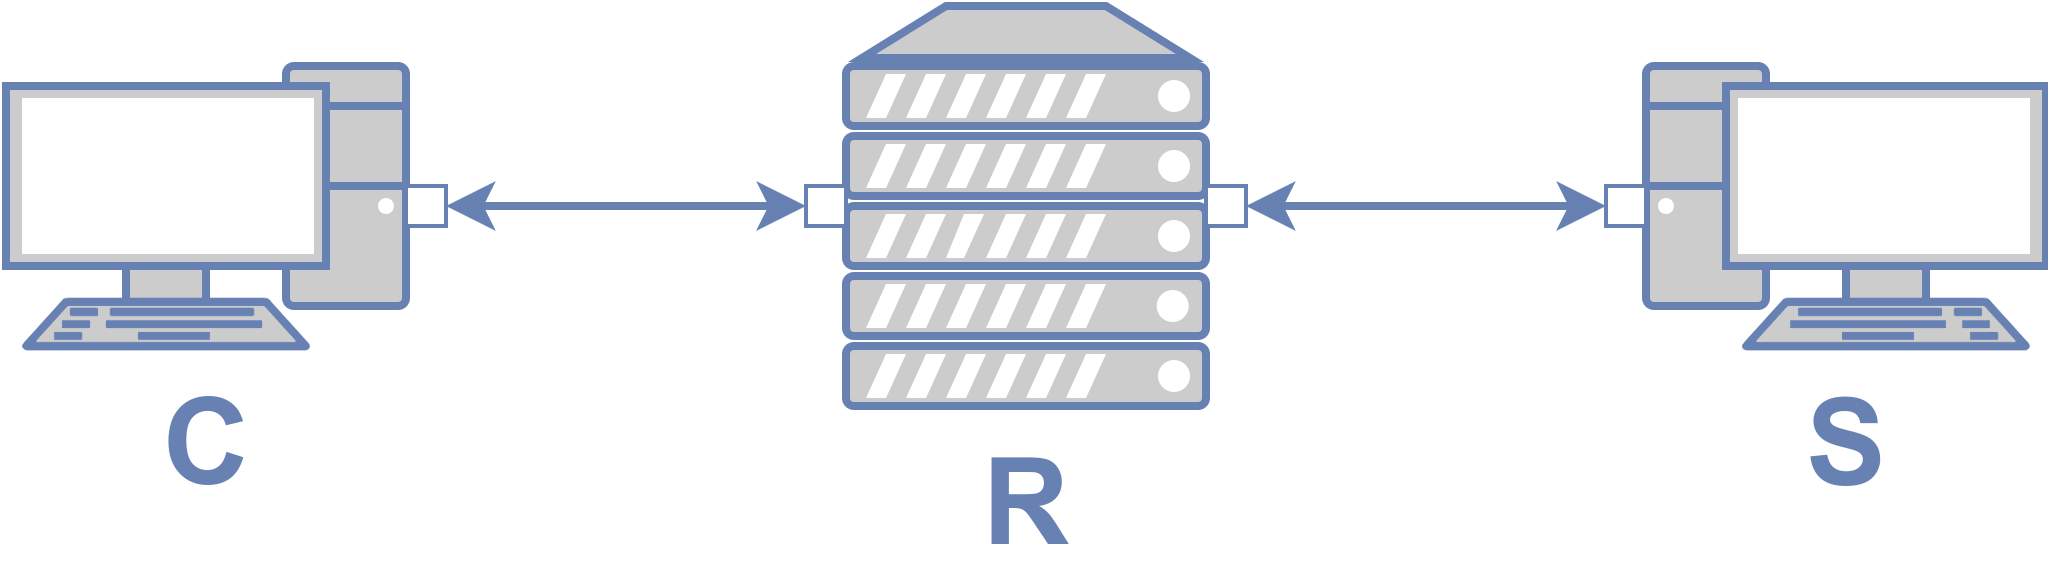
\includegraphics[width=6cm]{figures/testbed.png}
  \end{center}
  \vspace{-0.5cm}
  \caption{Performance Measurements Setups. C = Client. S = Server. MB = Middlebox.}
  \label{fig:perf_testbed}
    \vspace{-0.5cm}
\end{figure}

The traffic exchanged by client and server has to go through the NS first.

To evaluate TCPLS's functionalities, we rely on reproducible network
experimentations with Mininet~\cite{mininet}. Our objective is to compare the
behaviour of TCPLS with the state of the art, and to make it easily
reproducible for future works, as the quic implementations continue to evolve.

\subsection{Capability Comparison}

Table~\ref{table:tcplsvsquic} compares the features supported by
\tcp, \tls/\tcp, QUIC and \tcpls. QUIC and \tcpls are very similar in their
capabilities. They mainly differ in their semantic. \tcpls's semantic is to let
the applications make the decision, and we design its API to fulfill this goal.
That is, the meaning of \tcpls is to offer advanced, extensible and secure
transport-layer functionalities on top of \tcp, while exposing a simple but
powerful API to let the application composes the properties its transport should
have.

Note that several of the features suggested by \tcpls are also suggested on \tcp or
QUIC via research works such as a new socket API for explicit multipath for
\tcp\cite{hesmans2016enhanced}, or eBPF plugins in
QUIC~\cite{de2019pluginizing}.

\begin{table}
  \small
  \begin{tabular}{lcccc}
    \toprule
    & \tcp & \tls/\tcp & QUIC & \tcpls \\
    \midrule
    Transport reliability & \checkmark & \checkmark &
    \checkmark & \checkmark \\
    Message conf. and auth.&  \xmark & \checkmark & \checkmark & \checkmark \\
    Connection reliability &  \xmark & \xmark & (\checkmark) & (\checkmark) \\
    0-RTT & \checkmark & (\xmark) & \checkmark  & \checkmark \\
    Session Resumption & \xmark & \checkmark & \checkmark & \checkmark \\
    Connection Migration & \xmark & \xmark & \checkmark & \checkmark \\
    \multicolumn{5}{l}{Application-exposed features} \\
    \hspace{2em} Streams & \xmark & \xmark & \checkmark & \checkmark \\
    \hspace{2em} Happy eyeballs & \xmark & \xmark & \xmark & \checkmark \\
    \hspace{2em} Explicit Multipath & \xmark & \xmark & \xmark & \checkmark \\
    \hspace{2em} App-level Con. migration & \xmark & \xmark & \xmark & \checkmark \\
    \hspace{2em} Pluginization & \xmark & \xmark & \xmark & (\checkmark) \\
    Resilience to HOL blocking & \xmark & \xmark & \checkmark  & (\checkmark) \\
    Secure Connection Closing & \xmark &  \xmark & \checkmark & (\checkmark) \\
    \bottomrule
  \end{tabular}
  \caption{Protocol features comparison. (\xmark) means that the feature is
    available, but not straightforward to use. (\checkmark) means that the
  feature is partially available and under development.}
  \label{table:tcplsvsquic}
\end{table}

\subsection{Performance}
\label{sec:perf}


TCPLS vs QUIC vs TLS/TCP

Bar chart or/and tabular with throughput performance

\begin{figure}[!t]
   \begin{center}
     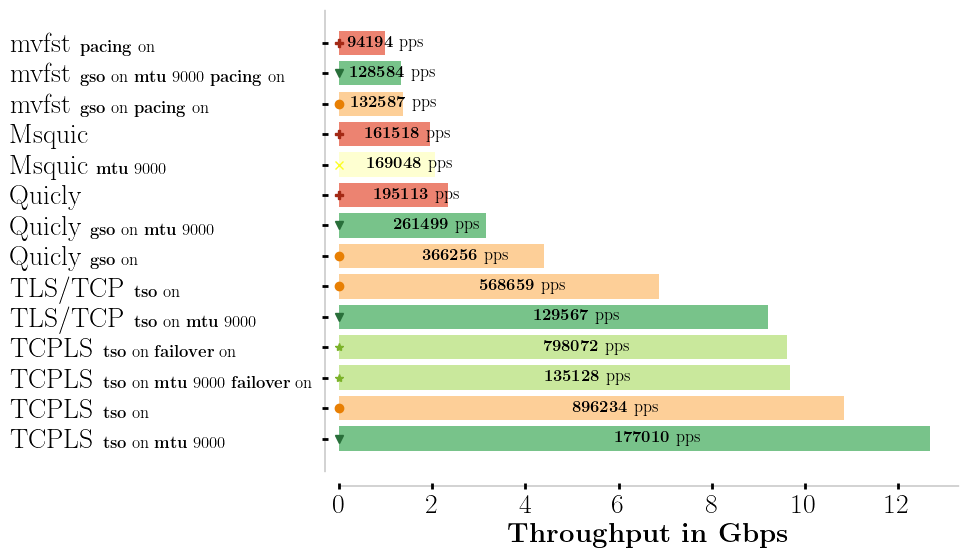
\includegraphics[width=\columnwidth]{figures/perf_analysis.png}
   \end{center}
   \caption{Throughput measurements of various QUIC stacks, TLS/TCP and TCPLS}
   \label{fig:perf}
\end{figure}

\subsection{Middlebox Interferences}

Montrer que TCPLS handshake et JOIN handshake passent/passent pas les middlebox,
discuter les implications

\subsection{Bandwidth Aggregation}

\begin{figure}[!t]
  \begin{center}
    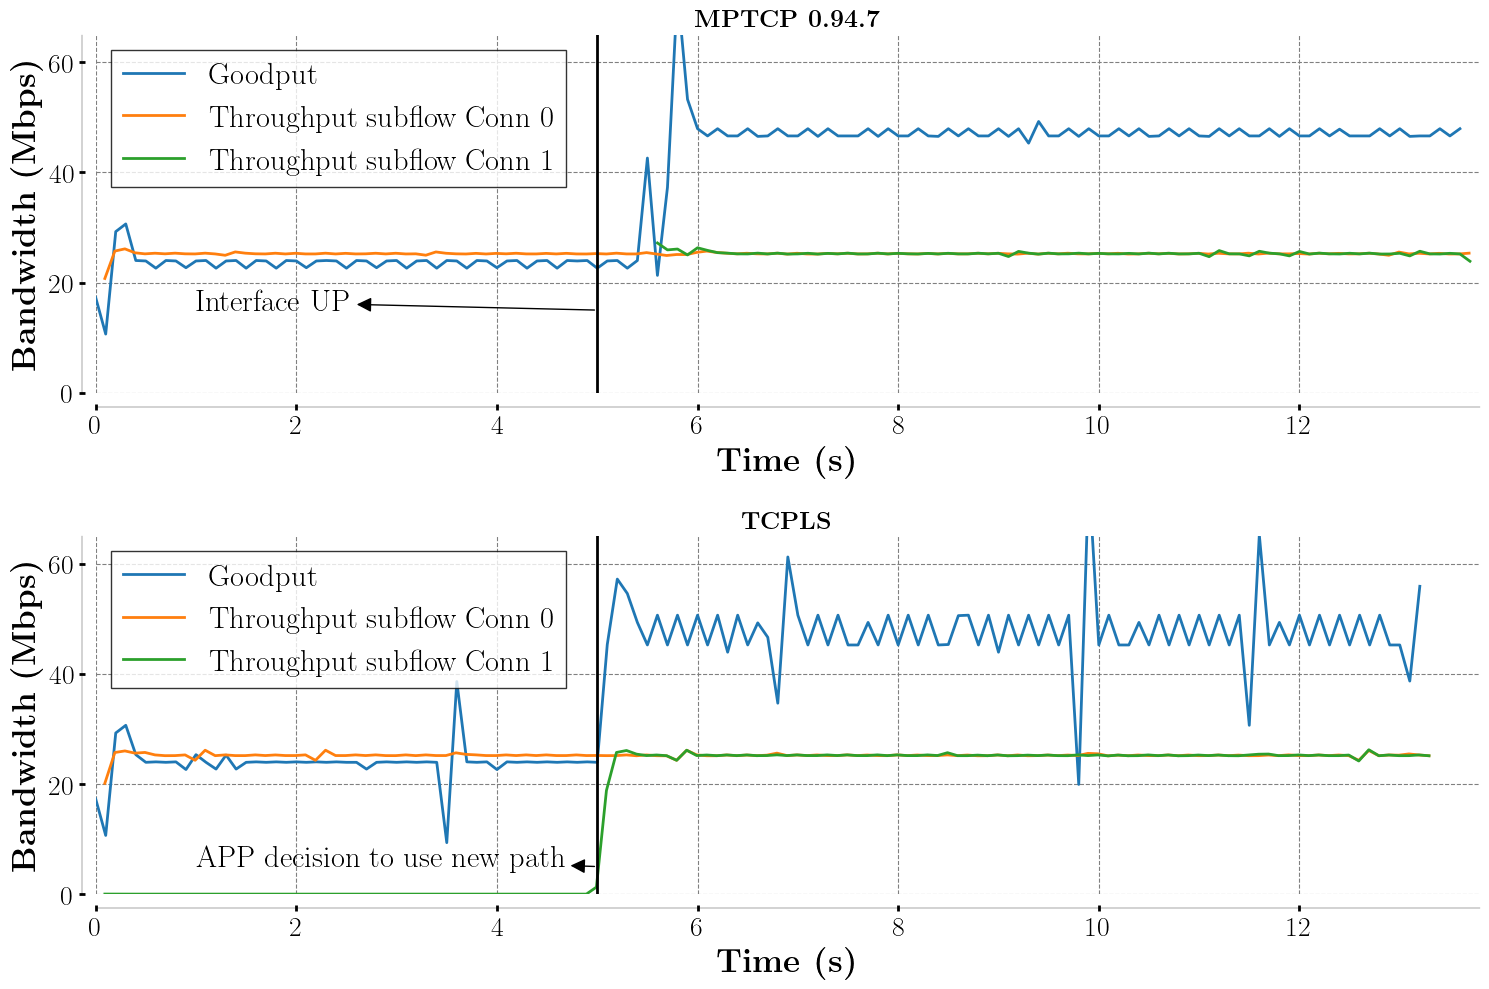
\includegraphics[width=\columnwidth]{figures/aggregate_dual.png}
  \end{center}
  \caption{Bandwidth aggregation comparison between MPTCP and TCPLS.}
\end{figure}

\subsection{Application-level migration}

Detailler pourquoi on a besoin du controle applicatif pour la migration, et à
quels cas du monde réels ils s'appliquent


Figure~\ref{fig:conn_migration} shows the result of an Application-level
connection migration demo using the API (i.e., it is left to the
application to decide when to migrate, and we expose a simplistic code flow to
perform it). In this experiment, we use an IPMininet network~\cite{ipmininet, jadin2020educational}
composed of a client and a server with a dual-stack of IPs. One path within the
network is composed of OSPF routers with IPv4 only, and one path is composed of
OSPF6 routers IPv6 only. We configure the bandwidth to 30Mbps, the lowest delay
to the v4 link. Our application
downloads a 60 MB file from a server and migrates to the v6 connection in
the middle of the download.

Triggering the connection migration involves chaining 5 API calls:
first, \texttt{tcpls\_handshake()} configured with handshake properties announcing a JOIN over the v6 connection id. Then, the creation of a new stream
\texttt{tcpls\_stream\_new()} for the v6 connection id, finally followed by the attachment of this new stream \texttt{tcpls\_streams\_attach()} and the secure closing of the v4 \tcp connection using \texttt{tcpls\_stream\_close()}. Following these events, the server seamlessly switches the path while looping over \texttt{tcpls\_send} to send the file content. Note that all the events trigger callbacks on the server side, to let the server react appropriately if other requirements need to be fulfilled.

\tcpls's application connection migration takes advantage of multipath to offer
a smooth handover to applications, which QUIC cannot do at the moment.

\begin{figure}[!t]
  \centering
  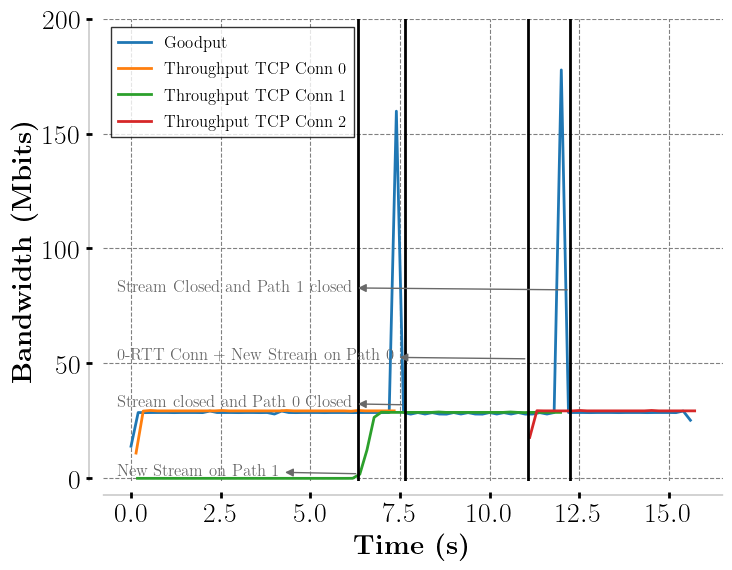
\includegraphics[width=6cm]{figures/migration.png}
  \caption{Application-level connection migration during a 60MB file download.}
  \label{fig:conn_migration}
\end{figure}

\subsection{Failover}

1) analyse du temps de recovery pour different type de cassure, et comparaison avec mptcp
2) discuter une propriété de "connection reliability" => ca casse, on restabilise le plus vite possible
3) montrer que le path manager est important pour cette propriété, et que ce n'est pas encore au point pour mptcp, mpquic, etc

Mptcp overhead: 1.0744997978210449
TCPLS overhead: 1.0994282363439873
MPTCP overhead/TCPLS overhead:              0.9773259975513828


\begin{figure}[!t]
  \begin{center}
    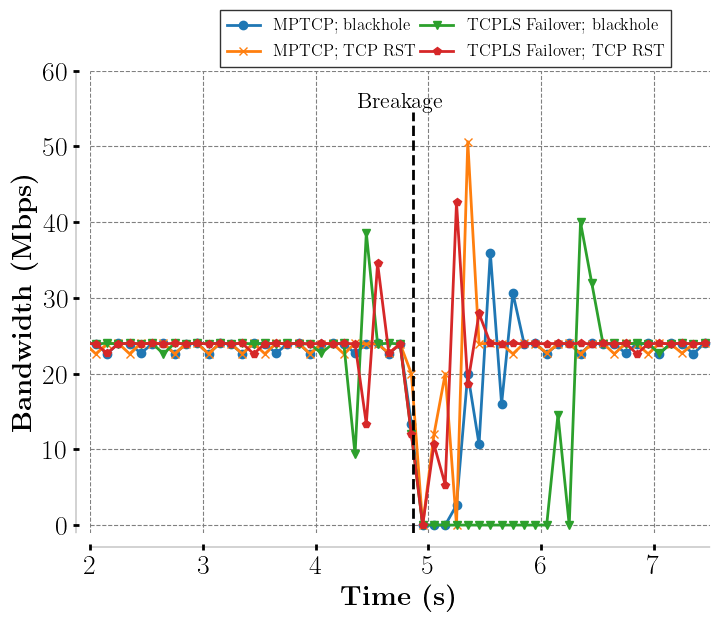
\includegraphics[width=6cm]{figures/breakage_analysis.png}
  \end{center}
  \caption{Recovery speed analysis.}
\end{figure}


\begin{figure}[!t]
  \begin{center}
    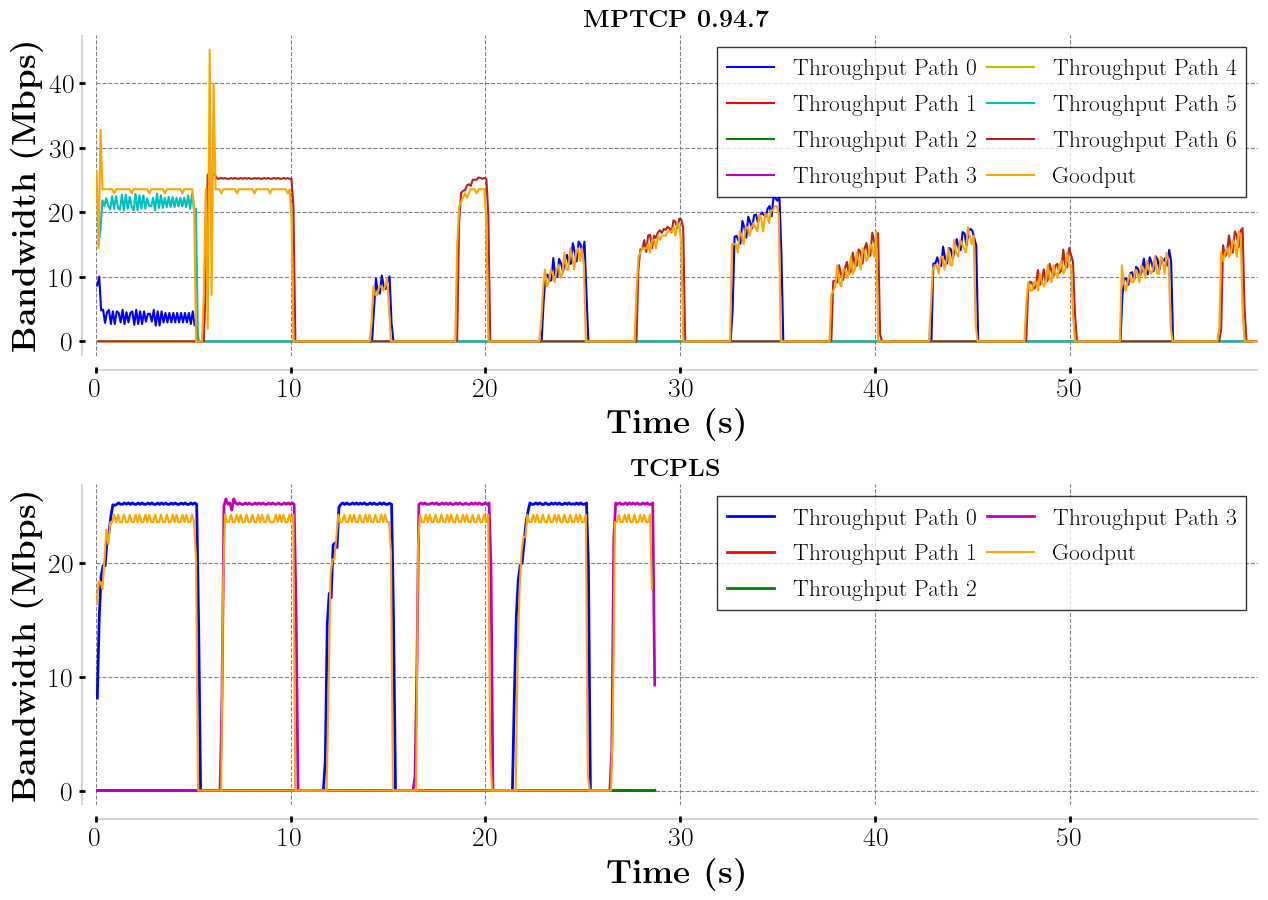
\includegraphics[width=6cm]{figures/tcpls_mptcp.png}
  \end{center}
  \caption{Connection reliability: influence of the path manager and congestion
  control.}
\end{figure}



\subsection{Congestion Control Injection}

Injecter un control de congestion, montrer que les perf s'améliorent
